\documentclass[12pt,letterpaper]{article}\usepackage[]{graphicx}\usepackage[]{color}
%% maxwidth is the original width if it is less than linewidth
%% otherwise use linewidth (to make sure the graphics do not exceed the margin)
\makeatletter
\def\maxwidth{ %
  \ifdim\Gin@nat@width>\linewidth
    \linewidth
  \else
    \Gin@nat@width
  \fi
}
\makeatother

\definecolor{fgcolor}{rgb}{0.345, 0.345, 0.345}
\newcommand{\hlnum}[1]{\textcolor[rgb]{0.686,0.059,0.569}{#1}}%
\newcommand{\hlstr}[1]{\textcolor[rgb]{0.192,0.494,0.8}{#1}}%
\newcommand{\hlcom}[1]{\textcolor[rgb]{0.678,0.584,0.686}{\textit{#1}}}%
\newcommand{\hlopt}[1]{\textcolor[rgb]{0,0,0}{#1}}%
\newcommand{\hlstd}[1]{\textcolor[rgb]{0.345,0.345,0.345}{#1}}%
\newcommand{\hlkwa}[1]{\textcolor[rgb]{0.161,0.373,0.58}{\textbf{#1}}}%
\newcommand{\hlkwb}[1]{\textcolor[rgb]{0.69,0.353,0.396}{#1}}%
\newcommand{\hlkwc}[1]{\textcolor[rgb]{0.333,0.667,0.333}{#1}}%
\newcommand{\hlkwd}[1]{\textcolor[rgb]{0.737,0.353,0.396}{\textbf{#1}}}%

\usepackage{framed}
\makeatletter
\newenvironment{kframe}{%
 \def\at@end@of@kframe{}%
 \ifinner\ifhmode%
  \def\at@end@of@kframe{\end{minipage}}%
  \begin{minipage}{\columnwidth}%
 \fi\fi%
 \def\FrameCommand##1{\hskip\@totalleftmargin \hskip-\fboxsep
 \colorbox{shadecolor}{##1}\hskip-\fboxsep
     % There is no \\@totalrightmargin, so:
     \hskip-\linewidth \hskip-\@totalleftmargin \hskip\columnwidth}%
 \MakeFramed {\advance\hsize-\width
   \@totalleftmargin\z@ \linewidth\hsize
   \@setminipage}}%
 {\par\unskip\endMakeFramed%
 \at@end@of@kframe}
\makeatother

\definecolor{shadecolor}{rgb}{.97, .97, .97}
\definecolor{messagecolor}{rgb}{0, 0, 0}
\definecolor{warningcolor}{rgb}{1, 0, 1}
\definecolor{errorcolor}{rgb}{1, 0, 0}
\newenvironment{knitrout}{}{} % an empty environment to be redefined in TeX

\usepackage{alltt}
\usepackage[left=2cm,right=2cm,top=2cm,bottom=2cm]{geometry}
\usepackage[ansinew]{inputenc}
\usepackage[spanish]{babel}
\usepackage{amsmath}
\usepackage{amsfonts}
\usepackage{amssymb}
\usepackage{dsfont}
\usepackage{multicol} 
\usepackage{subfigure}
\usepackage{graphicx}
\usepackage{float} 
\usepackage{verbatim} 
\usepackage[left=2cm,right=2cm,top=2cm,bottom=2cm]{geometry}
\usepackage{fancyhdr}
\pagestyle{fancy} 
\fancyhead[LO]{\leftmark}
\usepackage{caption}
\newtheorem{definicion}{Definci\'on}
\IfFileExists{upquote.sty}{\usepackage{upquote}}{}
\begin{document}

\begin{titlepage}
\setlength{\unitlength}{1 cm} %Especificar unidad de trabajo

\begin{center}
\textbf{{\large UNIVERSIDAD DE EL SALVADOR}\\ [0.50 cm]
{\large FACULTAD MULTIDISCIPLINARIA DE OCCIDENTE}\\ [0.50 cm]
{\large DEPARTAMENTO DE MATEM\'ATICA}}\\ [0.50 cm]

\begin{picture}(18,4)
 \put(7,0){
\includegraphics[width=4cm]{minerva.jpg}}
\end{picture}
\\[0.25 cm]

\textbf{{\large Licenciatura en Estad\'istica}\\ [1.25cm]
{\large Control Estad\'istico del Paquete R }\\ [2 cm]
%\setlength{\unitlength}{1 cm}
{\large  \textbf{''UNIDAD TRES"}}\\ [3 cm]
{\large Alumna:}\\
{\large Erika Beatr\'iz Guill\'en Pineda}\\ [2cm]
{\large Fecha de elaboraci\'on}\\
Santa Ana - \today }
\end{center}
\end{titlepage}

\newtheorem{teorema}{Teorema}
\newtheorem{prop}{Proposici\'on}[section]

\lhead{Pr?ctica 14}

\lfoot{LICENCIATURA EN ESTAD\'ISTICA}
\cfoot{UESOCC}
\rfoot{\thepage}
%\pagestyle{fancy} 

\setcounter{page}{1}
\newpage


\section{INTRODUCCI\'ON A LAS DISTRIBUCIONES DE PROBABILIDAD.}


La teor\'ia de la probabilidad y de variable aleatoria van a permitir establecer un amplio cat\'alogo de modelos te?ricos, tanto discretos como continuos, con los cuales se van a poder asimilar muchas de las situaciones de la vida real. El estudio de los modelos te\'oricos, incluyendo la caracterizaci\'on a trav\'es de sus par\'ametros, el c\'alculo de probabilidades en sus distintos formatos y la generaci\'on de n\'umeros aleatorios, van a facilitar enormemente el an?lisis de estas situaciones reales, algunos ejemplos de estos fen\'omenos son:\\

\begin{itemize}
  \item Si se contesta al azar un examen tipo test de 10 preguntas, donde cada una de ellas tiene 4 posibilidades siendo s\'olo una de ellas la correcta, Qu\'e n\'umero de aciertos es m\'as probable? 
  \item Se sabe que las bombillas de bajo consumo de 14 w tienen una vida media \'util de 10,000 horas, mientras que las bombillas cl\'asicas por incandescencia de 60 w tienen una vida media \'util de 1,000 horas. Si cada d?a se encienden unas 4 horas Cu\'al es la probabilidad de que despu\'es de un a\~o est\'an funcionando las dos?, ?ninguna de las dos?, ?al menos una de las dos? 
\end{itemize}

El primer problema a resolver ser\'a la elecci\'on del modelo te\'orico apropiado para cada caso en estudio. Para tener un buen manejo matem\'atico de las distintas situaciones que se puedan plantear dada la distinta naturaleza y la diversidad de los resultados que proporcionan los experimentos, se necesita realizar una abstracci\'on cuantificada del experimento. Esto lleva a una primera gran clasificaci\'on entre modelos de probabilidad discretos y continuos.\\

\\ Las probabilidades asociadas a cada uno de los valores de la variable aleatoria pueden ser organizadas como una distribuci\'on de probabilidad, expres\'andose mediante una tabla, una gr\'afica o una f\'ormula, denomin\'andose en este \'ultimo caso, a la regla de correspondencia-valores probabilidades, funci\'on de probabilidad.\\

Como sabemos, los n\'umeros aleatorios son descritos por una distribuci\'on. Esto es, alguna funci\'on la cual especifica la probabilidad que un n\'umero aleatorio este en alg\'un rango, por ejemplo P(a$<$X$<$b). Frecuentemente es dada por una densidad de probabilidad (en el caso continuo) o por una funci\'on masa de probabilidad P(X=x)=p(x) en el caso discreto. Con R podemos obtener n?meros seleccionados aleatoriamente de diferentes distribuciones, para ello s\'olo tenemos que familiarizarnos con los par\'ametros que hay que dar a las funciones tal como la media, o una proporci\'on, etc (dependiendo de la distribuci\'pn que se est\'e considerando y de lo que se est\'e analizando).\\

\newpage

\section{DISTRIBUCIONES DISCRETAS}


\begin{enumerate}
\item \textbf{Distribuci\'on Binomial.}

\begin{itemize}
\item \textbf{Par\'ametros}
\begin{center}
\item x = n?mero de ?xitos
\item size = n?mero de ensayos
\item p = proporci?n de ?xitos
\item lower.tail = TRUE P(X$<$=x)
\item lower.tail = FALSE P(X$>$=x) 
\item n = tama\~no de la muestra 
\end{center}
  
\item \textbf{Sintasis en R.}\\

\textbf{dbinom(x, size, prob, log = FALSE)}
\begin{knitrout}
\definecolor{shadecolor}{rgb}{0.969, 0.969, 0.969}\color{fgcolor}\begin{kframe}
\begin{alltt}
\hlkwd{dbinom}\hlstd{(}\hlnum{2}\hlstd{,} \hlnum{4}\hlstd{,} \hlnum{0.5}\hlstd{,} \hlkwc{log} \hlstd{=} \hlnum{FALSE}\hlstd{)}
\end{alltt}
\begin{verbatim}
## [1] 0.375
\end{verbatim}
\end{kframe}
\end{knitrout}

\textbf{pbinom(x, size, prob, lower.tail = TRUE, log.p = FALSE)}
\begin{knitrout}
\definecolor{shadecolor}{rgb}{0.969, 0.969, 0.969}\color{fgcolor}\begin{kframe}
\begin{alltt}
\hlkwd{pbinom}\hlstd{(}\hlnum{7}\hlstd{,} \hlnum{10}\hlstd{,} \hlnum{0.3}\hlstd{,} \hlkwc{lower.tail} \hlstd{=} \hlnum{TRUE}\hlstd{,} \hlkwc{log.p} \hlstd{=} \hlnum{FALSE}\hlstd{)}
\end{alltt}
\begin{verbatim}
## [1] 0.9984096
\end{verbatim}
\end{kframe}
\end{knitrout}

\textbf{qbinom(p, size, prob, lower.tail = TRUE, log.p = FALSE)}
\begin{knitrout}
\definecolor{shadecolor}{rgb}{0.969, 0.969, 0.969}\color{fgcolor}\begin{kframe}
\begin{alltt}
\hlkwd{qbinom}\hlstd{(}\hlnum{0.3}\hlstd{,} \hlnum{4}\hlstd{,} \hlnum{0.5}\hlstd{,} \hlkwc{lower.tail} \hlstd{=} \hlnum{TRUE}\hlstd{,} \hlkwc{log.p} \hlstd{=} \hlnum{FALSE}\hlstd{)}
\end{alltt}
\begin{verbatim}
## [1] 1
\end{verbatim}
\end{kframe}
\end{knitrout}

\textbf{rbinom(n, size, prob)} 
\begin{knitrout}
\definecolor{shadecolor}{rgb}{0.969, 0.969, 0.969}\color{fgcolor}\begin{kframe}
\begin{alltt}
\hlkwd{rbinom}\hlstd{(}\hlnum{10}\hlstd{,} \hlnum{4}\hlstd{,} \hlnum{0.3}\hlstd{)}
\end{alltt}
\begin{verbatim}
##  [1] 0 2 0 1 0 3 2 1 3 1
\end{verbatim}
\end{kframe}
\end{knitrout}

\end{itemize}

\item  \textbf{Distribuci\'on Geom\'etrica}
\begin{itemize}
\item \textbf{Par\'ametros}
\begin{center}
x = ensayos necesarios para obtener el primer \'exito\\
p = proporci?n de ?xitos\\
lower.tail = TRUE P(X$<$=x)\\
lower.tail = FALSE P(X$>$=x)\\ 
n = tama\~no de la muestra 
\end{center}
  
\item \textbf{Sintasis en R.}\\

\textbf{dgeom(x, prob, log = FALSE)}
\begin{knitrout}
\definecolor{shadecolor}{rgb}{0.969, 0.969, 0.969}\color{fgcolor}\begin{kframe}
\begin{alltt}
\hlkwd{dgeom}\hlstd{(}\hlnum{4}\hlstd{,} \hlnum{0.25}\hlstd{,} \hlkwc{log} \hlstd{=} \hlnum{FALSE}\hlstd{)}
\end{alltt}
\begin{verbatim}
## [1] 0.07910156
\end{verbatim}
\end{kframe}
\end{knitrout}

\textbf{pgeom(x, prob, lower.tail = TRUE, log.p = FALSE)}
\begin{knitrout}
\definecolor{shadecolor}{rgb}{0.969, 0.969, 0.969}\color{fgcolor}\begin{kframe}
\begin{alltt}
\hlkwd{pgeom}\hlstd{(}\hlnum{4}\hlstd{,} \hlnum{0.25}\hlstd{,} \hlkwc{lower.tail} \hlstd{=} \hlnum{TRUE}\hlstd{,} \hlkwc{log.p} \hlstd{=} \hlnum{FALSE}\hlstd{)}
\end{alltt}
\begin{verbatim}
## [1] 0.7626953
\end{verbatim}
\end{kframe}
\end{knitrout}

\textbf{qgeom(p, prob, lower.tail = TRUE, log.p = FALSE)}
\begin{knitrout}
\definecolor{shadecolor}{rgb}{0.969, 0.969, 0.969}\color{fgcolor}\begin{kframe}
\begin{alltt}
\hlkwd{qgeom}\hlstd{(}\hlnum{0.75}\hlstd{,} \hlnum{0.25}\hlstd{,} \hlkwc{lower.tail} \hlstd{=} \hlnum{TRUE}\hlstd{,} \hlkwc{log.p} \hlstd{=} \hlnum{FALSE}\hlstd{)}
\end{alltt}
\begin{verbatim}
## [1] 4
\end{verbatim}
\end{kframe}
\end{knitrout}

\textbf{rgeom(n, prob)}
\begin{knitrout}
\definecolor{shadecolor}{rgb}{0.969, 0.969, 0.969}\color{fgcolor}\begin{kframe}
\begin{alltt}
\hlkwd{rgeom}\hlstd{(}\hlnum{15}\hlstd{,} \hlnum{0.25}\hlstd{)}
\end{alltt}
\begin{verbatim}
##  [1] 4 0 5 0 0 7 7 1 1 6 3 2 3 5 0
\end{verbatim}
\end{kframe}
\end{knitrout}
\end{itemize}

\item  \textbf{Distribuci\'on Hipergeom\'etrica}
\begin{itemize}
\item \textbf{Par\'ametros}
\begin{center}
\itm x = objetos seleccionados tipo m (primer tipo)
\item m = total de objetos (primer tipo)
\item n = total de objetos (segundo tipo)
\item y = el n\'umero total de objetos seleccionados primer tipo y segundo tipo
\item size = tama\~no de la muestra\\ 
\end{center}
  
\item \textbf{Sintasis en R}

\textbf{dhyper(x, m, n, y, log = FALSE)}
\begin{knitrout}
\definecolor{shadecolor}{rgb}{0.969, 0.969, 0.969}\color{fgcolor}\begin{kframe}
\begin{alltt}
\hlkwd{dhyper}\hlstd{(}\hlnum{8}\hlstd{,} \hlnum{8}\hlstd{,} \hlnum{5}\hlstd{,} \hlnum{13}\hlstd{,} \hlkwc{log} \hlstd{=} \hlnum{FALSE}\hlstd{)}
\end{alltt}
\begin{verbatim}
## [1] 1
\end{verbatim}
\end{kframe}
\end{knitrout}

\textbf{phyper(x, m, n, y, lower.tail = TRUE, log.p = FALSE)}
\begin{knitrout}
\definecolor{shadecolor}{rgb}{0.969, 0.969, 0.969}\color{fgcolor}\begin{kframe}
\begin{alltt}
\hlkwd{phyper}\hlstd{(}\hlnum{5}\hlstd{,} \hlnum{5}\hlstd{,} \hlnum{14}\hlstd{,} \hlnum{19}\hlstd{,} \hlkwc{lower.tail} \hlstd{=} \hlnum{TRUE}\hlstd{,} \hlkwc{log.p} \hlstd{=} \hlnum{FALSE}\hlstd{)}
\end{alltt}
\begin{verbatim}
## [1] 1
\end{verbatim}
\end{kframe}
\end{knitrout}

\textbf{qhyper(p, m, n, y, lower.tail = TRUE, log.p = FALSE)}
\begin{knitrout}
\definecolor{shadecolor}{rgb}{0.969, 0.969, 0.969}\color{fgcolor}\begin{kframe}
\begin{alltt}
\hlkwd{qhyper}\hlstd{(}\hlnum{0.25}\hlstd{,} \hlnum{6}\hlstd{,} \hlnum{5}\hlstd{,} \hlnum{11}\hlstd{,} \hlkwc{lower.tail} \hlstd{=} \hlnum{TRUE}\hlstd{,} \hlkwc{log.p} \hlstd{=} \hlnum{FALSE}\hlstd{)}
\end{alltt}
\begin{verbatim}
## [1] 6
\end{verbatim}
\end{kframe}
\end{knitrout}

\textbf{rhyper(size, n, m, n,y)}
\begin{knitrout}
\definecolor{shadecolor}{rgb}{0.969, 0.969, 0.969}\color{fgcolor}\begin{kframe}
\begin{alltt}
\hlkwd{rhyper}\hlstd{(}\hlnum{20}\hlstd{,} \hlnum{4}\hlstd{,} \hlnum{6}\hlstd{,} \hlnum{10}\hlstd{)}
\end{alltt}
\begin{verbatim}
##  [1] 4 4 4 4 4 4 4 4 4 4 4 4 4 4 4 4 4 4 4 4
\end{verbatim}
\end{kframe}
\end{knitrout}
\end{itemize}

\item  \textbf{Distribuci\'on Poisson}
\begin{itemize}
\item \textbf{Par\'ametros}
\begin{center}
\item x = valor cualqueira\\
\item p = probabilidad \\
\item lambda = media de la distribuci\'on\\
\tem size = tama\~no de la muestra\\ 
\end{center}
  
\item \textbf{Sintasis en R.}\\

\textbf{dpois(x, lambda, log = FALSE)}
\begin{knitrout}
\definecolor{shadecolor}{rgb}{0.969, 0.969, 0.969}\color{fgcolor}\begin{kframe}
\begin{alltt}
\hlkwd{dpois}\hlstd{(}\hlnum{3}\hlstd{,} \hlnum{0.8}\hlstd{,} \hlkwc{log} \hlstd{=} \hlnum{FALSE}\hlstd{)}
\end{alltt}
\begin{verbatim}
## [1] 0.03834274
\end{verbatim}
\end{kframe}
\end{knitrout}

\textbf{ppois(x, lambda, lower.tail = TRUE, log.p = FALSE)}
\begin{knitrout}
\definecolor{shadecolor}{rgb}{0.969, 0.969, 0.969}\color{fgcolor}\begin{kframe}
\begin{alltt}
\hlkwd{ppois}\hlstd{(}\hlnum{3}\hlstd{,} \hlnum{7.5}\hlstd{,} \hlkwc{lower.tail} \hlstd{=} \hlnum{TRUE}\hlstd{,} \hlkwc{log.p} \hlstd{=} \hlnum{FALSE}\hlstd{)}
\end{alltt}
\begin{verbatim}
## [1] 0.05914546
\end{verbatim}
\end{kframe}
\end{knitrout}

\textbf{qpois(p, lambda, lower.tail = TRUE, log.p = FALSE)}
\begin{knitrout}
\definecolor{shadecolor}{rgb}{0.969, 0.969, 0.969}\color{fgcolor}\begin{kframe}
\begin{alltt}
\hlkwd{qpois}\hlstd{(}\hlnum{0.5162}\hlstd{,} \hlnum{3.75}\hlstd{,} \hlkwc{lower.tail} \hlstd{=} \hlnum{TRUE}\hlstd{,} \hlkwc{log.p} \hlstd{=} \hlnum{FALSE}\hlstd{)}
\end{alltt}
\begin{verbatim}
## [1] 4
\end{verbatim}
\end{kframe}
\end{knitrout}
\end{itemize}
\end{itemize}
\end{enumerate}

Para cada una de las distribuciones discretas o continuas est?n disponibles las siguientes opciones:
\begin{itemize}
\item Gr\'afica de la distribuci\'on: Genera la gr\'afica de la funci\'on de probabilidad.
\item Probabilidades: Determina la probabilidad deque la variable tome un valor dado. 
\item Probabilidades Acumuladas: Calcula bien el valor de P(X$<$=x)(cola de la izquierda), o bien, P(X$>$x)(cola de la derecha) para cada cuantil(q) de X.
\item Cuantiles: Permite calcular el valor de la variable que deja a derecha o a izquierda (seg\'un se seleccione) una determinada probabilidad. 
\item Muestra de la distribuci\'on: Genera muestras aleatorias extra\'idas de la distribuci\'on. 
\end{itemize}

El Paquete R proporciona 4 funciones para cada distribuci\'on (ya sea continua o discreta) que pueden usarse escribiendo el nombre de la distribuci\'on, anteponi?ndole una d, si se quiere la funci\'on de densidad o la probabilidad de que la variable tome el valor especificado en x, es decir P(X=x); una p para la funci\'on de distribuci?n acumulada, es decir P(X$<$=x); una q para los cuantiles, es decir, el valor x de la distribuci\'on acumulada que deja un \'area igual p P(X$<$=x)=p, y una r para generar una muestra aleatoria de la distribuci\'on; \'unicamente hay que tener en cuenta la sintaxis presentada en el cuadro anterior.


\section{C\'ALCULO DE PROBABILIDADES.}

\begin{itemize}
\item \textbf{Ejemplo 1:}\\

Si un estudiante responde al azar a un examen de 8 preguntas de verdadero o falso.
\begin{description}
\item a) Cu\'al es la probabilidad de que acierte 4? P[X=4]
 \end{description}
La variable X="n\'umero de aciertos" sigue una distribuci\'on Binomial de par\'ametros n = 8 y p=1$/$2(p probabilidad de ?xito).
\begin{knitrout}
\definecolor{shadecolor}{rgb}{0.969, 0.969, 0.969}\color{fgcolor}\begin{kframe}
\begin{alltt}
\hlcom{# Usando la funciones propias de R}

\hlkwd{dbinom}\hlstd{(}\hlnum{4}\hlstd{,}\hlnum{8}\hlstd{,}\hlnum{0.5}\hlstd{)}
\end{alltt}
\begin{verbatim}
## [1] 0.2734375
\end{verbatim}
\begin{alltt}
\hlcom{# dbinom calcula la probabilidad en un valor concreto }
\end{alltt}
\end{kframe}
\end{knitrout}

\begin{description}
   \item b) Cu\'al es la probabilidad de que acierte a lo sumo 2? P[X$<$=2]
\begin{knitrout}
\definecolor{shadecolor}{rgb}{0.969, 0.969, 0.969}\color{fgcolor}\begin{kframe}
\begin{alltt}
\hlstd{x} \hlkwb{<-} \hlnum{2}\hlstd{; n}\hlkwb{=}\hlnum{8}\hlstd{; p}\hlkwb{=}\hlnum{1}\hlopt{/}\hlnum{2}

\hlkwd{pbinom}\hlstd{(x,} \hlkwc{size} \hlstd{= n,} \hlkwc{prob} \hlstd{= p,} \hlkwc{lower.tail}\hlstd{=}\hlnum{TRUE}\hlstd{)}
\end{alltt}
\begin{verbatim}
## [1] 0.1445313
\end{verbatim}
\begin{alltt}
\hlcom{# pbinom es la funcion de distribucion acumulada }
\end{alltt}
\end{kframe}
\end{knitrout}
 \end{description}
 
\begin{description}
   \item b) ?Cu\'al es la probabilidad de que acierte 5 o m?s? P[X$>$=5]
\begin{knitrout}
\definecolor{shadecolor}{rgb}{0.969, 0.969, 0.969}\color{fgcolor}\begin{kframe}
\begin{alltt}
\hlstd{x} \hlkwb{<-} \hlnum{4}\hlstd{; n}\hlkwb{=}\hlnum{8}\hlstd{; p}\hlkwb{=}\hlnum{1}\hlopt{/}\hlnum{2}

\hlcom{#primera forma}

\hlstd{F} \hlkwb{<-} \hlnum{1} \hlopt{-} \hlkwd{pbinom}\hlstd{(x, n, p,} \hlkwc{lower.tail}\hlstd{=}\hlnum{TRUE}\hlstd{); F}
\end{alltt}
\begin{verbatim}
## [1] 0.3632813
\end{verbatim}
\end{kframe}
\end{knitrout}
\begin{knitrout}
\definecolor{shadecolor}{rgb}{0.969, 0.969, 0.969}\color{fgcolor}\begin{kframe}
\begin{alltt}
\hlcom{#segunda forma}

\hlkwd{pbinom}\hlstd{(}\hlnum{4}\hlstd{,} \hlkwc{size}\hlstd{=}\hlnum{8}\hlstd{,} \hlkwc{prob}\hlstd{=}\hlnum{0.5}\hlstd{,} \hlkwc{lower.tail}\hlstd{=}\hlnum{FALSE}\hlstd{)}
\end{alltt}
\begin{verbatim}
## [1] 0.3632813
\end{verbatim}
\end{kframe}
\end{knitrout}
\end{description}

\item \textbf{Ejemplo 2:}\\

Una cierta \'area de Estados Unidos es afectada, en promedio, por 6 huracanes al a?o. Encuentre la probabilidad de que en un determinado a?o esta \'area sea afectada por:
\begin{description}
  \item a) Menos de 4 huracanes.P[X$<$4]=F(3)
\end{description}
Se define la variable X = "n\'umero de huracanes por a\~o" y asumiendo que dicha variable tiene una distribuci\'on de Poisson de par?metro lambda igual a 6, porque describe el n\'umero de \'exitos por unidad de tiempo y porque son independientes del tiempo desde el \'ultimo evento. Se calcular\'an ahora las probabilidades: 
\begin{knitrout}
\definecolor{shadecolor}{rgb}{0.969, 0.969, 0.969}\color{fgcolor}\begin{kframe}
\begin{alltt}
\hlstd{x} \hlkwb{<-} \hlnum{3}\hlstd{; mu} \hlkwb{<-} \hlnum{6}

\hlkwd{ppois}\hlstd{(x,} \hlkwc{lambda} \hlstd{= mu,} \hlkwc{lower.tail}\hlstd{=}\hlnum{TRUE}\hlstd{)}
\end{alltt}
\begin{verbatim}
## [1] 0.1512039
\end{verbatim}
\end{kframe}
\end{knitrout}
\begin{description}
\item b) Entre 6 y 8 huracanes.P[6$<$=X$<$=8]=P[X$<$=8]-P[X$<$=5]=F(8)-F(5)
\end{description}
Para calcular la probabilidad de que ocurran entre 6 y 8 huracanes, se pueden sumar las probabilidades P(X=6)+P(X=7)+P(X=8)

\textbf{# primera forma}
\begin{knitrout}
\definecolor{shadecolor}{rgb}{0.969, 0.969, 0.969}\color{fgcolor}\begin{kframe}
\begin{alltt}
\hlkwd{sum}\hlstd{(}\hlkwd{dpois}\hlstd{(}\hlkwd{c}\hlstd{(}\hlnum{6}\hlstd{,}\hlnum{7}\hlstd{,}\hlnum{8}\hlstd{),}\hlkwc{lambda} \hlstd{=} \hlnum{6}\hlstd{))}
\end{alltt}
\begin{verbatim}
## [1] 0.4015579
\end{verbatim}
\end{kframe}
\end{knitrout}

\textbf{# segunda forma}
\begin{knitrout}
\definecolor{shadecolor}{rgb}{0.969, 0.969, 0.969}\color{fgcolor}\begin{kframe}
\begin{alltt}
\hlcom{# O restar las probabilidades acumuladas, con la opcion Cola izquierda, }
\hlcom{# P(X<=8)-P(X<=5).Como antes se realizan en primer lugar las probabilidades }
\hlcom{# acumuladas y se restan los resultados obtenidos:}

\hlstd{F8} \hlkwb{<-} \hlkwd{ppois}\hlstd{(}\hlnum{8}\hlstd{,} \hlkwc{lambda} \hlstd{=} \hlnum{6}\hlstd{,} \hlkwc{lower.tail}\hlstd{=}\hlnum{TRUE}\hlstd{)}
\hlstd{F5} \hlkwb{<-} \hlkwd{ppois}\hlstd{(}\hlnum{5}\hlstd{,}\hlkwc{lambda} \hlstd{=} \hlnum{6}\hlstd{,} \hlkwc{lower.tail}\hlstd{=}\hlnum{TRUE}\hlstd{)}
\hlstd{F8} \hlopt{-} \hlstd{F5}
\end{alltt}
\begin{verbatim}
## [1] 0.4015579
\end{verbatim}
\end{kframe}
\end{knitrout}
\begin{description}
  \item c) Represente gr\'aficamente la funci\'on de probabilidad de la variable aleatoria que mide el n\'umero de huracanes por a\~no.
\end{description}

\begin{knitrout}
\definecolor{shadecolor}{rgb}{0.969, 0.969, 0.969}\color{fgcolor}\begin{kframe}
\begin{alltt}
\hlstd{n} \hlkwb{<-} \hlnum{30}

\hlcom{# genera 30 valores de una distribucion de Poisson con lambda igual a 6 }

\hlstd{x} \hlkwb{<-} \hlkwd{rpois}\hlstd{(n,} \hlkwc{lambda}\hlstd{=mu)}
\hlstd{x} \hlkwb{<-} \hlkwd{rpois}\hlstd{(}\hlnum{30}\hlstd{,} \hlkwc{lambda}\hlstd{=}\hlnum{6}\hlstd{)}

\hlcom{#calcula las probabilidades para cada valor generado }

\hlstd{y} \hlkwb{<-} \hlkwd{dpois}\hlstd{(x,} \hlkwc{lambda}\hlstd{=mu)}
\hlstd{y} \hlkwb{<-} \hlkwd{dpois}\hlstd{(x,} \hlkwc{lambda}\hlstd{=}\hlnum{6}\hlstd{)}


\hlcom{#genera el grafico de distribuci?n}

\hlkwd{plot}\hlstd{(x, y,} \hlkwc{xlab}\hlstd{=}\hlstr{"x"}\hlstd{,} \hlkwc{ylab}\hlstd{=}\hlstr{"Funcion de probalidad"}\hlstd{,} \hlkwc{main}\hlstd{=}\hlstr{"Distribucion 
     de Poisson: lambda = 6"}\hlstd{,} \hlkwc{type}\hlstd{=}\hlstr{"h"}\hlstd{)}

\hlcom{#une los puntos a las lineas}

\hlkwd{points}\hlstd{(x, y,} \hlkwc{pch}\hlstd{=}\hlnum{21}\hlstd{)}
\end{alltt}
\end{kframe}
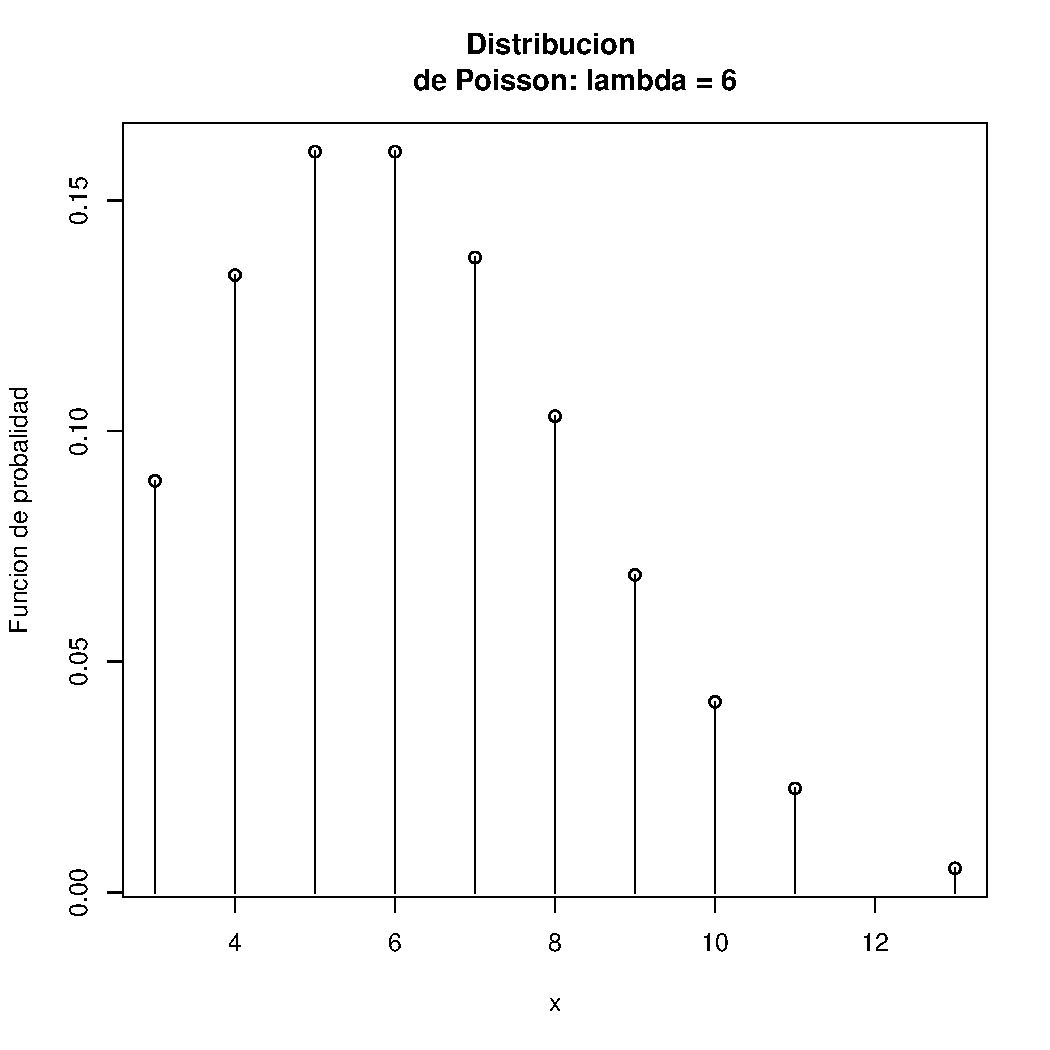
\includegraphics[width=\maxwidth]{figure/unnamed-chunk-23-1} 

\end{knitrout}
\item \textbf{Ejemplo 3:}\\

En un juego se disponen 15 globos llenos de agua, de los que 4 tienen premio. Los participantes en el juego, con los ojos vendados, golpean los globos con un bate por orden hasta que cada uno consigue romper 2. 

\begin{description}
  \item a) Cu\'al es la probabilidad de que el primer participante consiga un premio?
\end{description}  

mero de premios conseguidos entre 2 posibles" sigue una distribuci\'on hipergeom\'etrica de par\'ametros m=11, n=4, K=2. 

\begin{knitrout}
\definecolor{shadecolor}{rgb}{0.969, 0.969, 0.969}\color{fgcolor}\begin{kframe}
\begin{alltt}
\hlstd{x} \hlkwb{<-} \hlnum{0}\hlopt{:}\hlnum{2}\hlstd{; m} \hlkwb{=} \hlnum{11}\hlstd{; n} \hlkwb{<-} \hlnum{4}\hlstd{; k}\hlkwb{=}\hlnum{2}

\hlcom{# x define el n\textbackslash{}'umero de globos con premio }
\hlcom{# se construye la distribucion de frecuencias del numero de premios }

\hlstd{Tabla} \hlkwb{<-} \hlkwd{data.frame}\hlstd{(}\hlkwc{Probabilidad}\hlstd{=}\hlkwd{dhyper}\hlstd{(x, m, n, k))}
\hlkwd{rownames}\hlstd{(Tabla)} \hlkwb{<-} \hlkwd{c}\hlstd{(}\hlstr{"Ningun premio"}\hlstd{,}\hlstr{"Solamente uno"}\hlstd{,} \hlstr{"Dos premios"}\hlstd{)}
\hlstd{Tabla}
\end{alltt}
\begin{verbatim}
##               Probabilidad
## Ningun premio   0.05714286
## Solamente uno   0.41904762
## Dos premios     0.52380952
\end{verbatim}
\end{kframe}
\end{knitrout}

\begin{description}
  \item b) Si el primer participante ha conseguido s\'olo un premio, cu\'al es la probabilidad de que el segundo participante consiga otro? 
\end{description}

Para el segundo participante la variable seguir\'a una hipergeom\'etrica de par\'ametros m= 10, n= 3 y k= 2, 

\begin{knitrout}
\definecolor{shadecolor}{rgb}{0.969, 0.969, 0.969}\color{fgcolor}\begin{kframe}
\begin{alltt}
\hlstd{x} \hlkwb{=} \hlnum{1}\hlstd{; m}\hlkwb{=} \hlnum{10}\hlstd{; n}\hlkwb{=} \hlnum{3}\hlstd{; k}\hlkwb{=} \hlnum{2}\hlstd{;}
\hlkwd{dhyper}\hlstd{(x, m, n, k)}
\end{alltt}
\begin{verbatim}
## [1] 0.3846154
\end{verbatim}
\end{kframe}
\end{knitrout}

\item \textbf{Ejemplo 4:}\\
Un vendedor de alarmas de hogar tiene \'exito enuna casa de cada diez que visita. 
Calcula:

\begin{description}
\item a) La probabilidad de que en un da determinado consiga vender la primera alarma en la sexta casa que visita. 
\end{description}

Se define la variable X="n\'umero de casas que visita antes de conseguir vender la primera alarma", que sigue una distribuci\'on Geom\'etrica con Probabilidad de \'exito=0.1 \\

Habr\'ia que calcular la probabilidadde que tenga 5 fracasos antes del primer \'exito, obteniendo de la tabla la probabilidad P(X=5)=0.059049

\begin{knitrout}
\definecolor{shadecolor}{rgb}{0.969, 0.969, 0.969}\color{fgcolor}\begin{kframe}
\begin{alltt}
\hlcom{# x define el n\textbackslash{}'umero de intentos fallidos}

\hlstd{x} \hlkwb{<-} \hlnum{0}\hlopt{:}\hlnum{5}\hlstd{; p}\hlkwb{=}\hlnum{0.1}

\hlcom{# creando la tabla de distribucion de frecuencias del n\textbackslash{}'umero de intentos }
\hlcom{# fallidos antes de obtener la primera venta. }

\hlstd{Tabla} \hlkwb{<-} \hlkwd{data.frame}\hlstd{(}\hlkwc{Probabilidad}\hlstd{=}\hlkwd{dgeom}\hlstd{(x,} \hlkwc{prob}\hlstd{=p))}

\hlcom{# nombrando las filas de la distribuci\textbackslash{}'on de frecuencias}

\hlkwd{rownames}\hlstd{(Tabla)} \hlkwb{<-} \hlkwd{c}\hlstd{(}\hlstr{"Venta en el primer intento"}\hlstd{,}
                     \hlstr{"Venta en el segundo intento"}\hlstd{,}
                     \hlstr{"Venta en el tercer intento"}\hlstd{,}
                     \hlstr{"Venta en el cuarto intento"}\hlstd{,}
                     \hlstr{"Venta en el quinto intento"}\hlstd{,}
                     \hlstr{"Venta en el sexto intento"}\hlstd{)}

\hlstd{Tabla}
\end{alltt}
\begin{verbatim}
##                             Probabilidad
## Venta en el primer intento      0.100000
## Venta en el segundo intento     0.090000
## Venta en el tercer intento      0.081000
## Venta en el cuarto intento      0.072900
## Venta en el quinto intento      0.065610
## Venta en el sexto intento       0.059049
\end{verbatim}
\end{kframe}
\end{knitrout}

\begin{description}
  \item b) La probabilidad de que no venda ninguna despu\'es de siete viviendas visitadas. 
\end{description}

La variable X="n\'umero de alarmas vendidas en 7 viviendas" sigue una distribuci\'on Binomial con n=7 Ensayos binomiales y Probabilidad de \'exito p=0.1, luego en nuestro caso se tiene P(X=0)=0.4782969

\begin{knitrout}
\definecolor{shadecolor}{rgb}{0.969, 0.969, 0.969}\color{fgcolor}\begin{kframe}
\begin{alltt}
\hlstd{x}\hlkwb{=}\hlnum{0}\hlstd{; n}\hlkwb{=}\hlnum{7}\hlstd{; p}\hlkwb{=}\hlnum{0.1}
\hlkwd{dbinom}\hlstd{(x, n, p,} \hlkwc{log} \hlstd{=} \hlnum{FALSE}\hlstd{)}
\end{alltt}
\begin{verbatim}
## [1] 0.4782969
\end{verbatim}
\end{kframe}
\end{knitrout}

\begin{description}
  \item c) Si se plantea vender tres alarmas, cu\'al es la probabilidad deque consiga su objetivo en la octava vivienda que visita?  
\end{description}

Para abordar esta cuesti\'on, se define la variable Y= "n\'umero de casas que visita antes de conseguir vender la tercera alarma. Esta variable sigue una distribuci\'on Binomial Negativa de par\'ametros N\'umero de \'exitos= 3, Probabilidad de \'exito p=0.1, de donde: P(Y=5)=0.01240029

\begin{knitrout}
\definecolor{shadecolor}{rgb}{0.969, 0.969, 0.969}\color{fgcolor}\begin{kframe}
\begin{alltt}
\hlstd{y} \hlkwb{<-} \hlnum{0}\hlopt{:}\hlnum{5}\hlstd{; r}\hlkwb{=}\hlnum{3}\hlstd{; p} \hlkwb{<-} \hlnum{0.1}

\hlstd{Tabla} \hlkwb{<-} \hlkwd{data.frame}\hlstd{(}\hlkwc{Probabilidad}\hlstd{=}\hlkwd{dnbinom}\hlstd{(y,} \hlkwc{size}\hlstd{=r,} \hlkwc{prob}\hlstd{=p))}

\hlkwd{rownames}\hlstd{(Tabla)} \hlkwb{<-} \hlnum{0}\hlopt{:}\hlnum{5}

\hlstd{Tabla}
\end{alltt}
\begin{verbatim}
##   Probabilidad
## 0   0.00100000
## 1   0.00270000
## 2   0.00486000
## 3   0.00729000
## 4   0.00984150
## 5   0.01240029
\end{verbatim}
\end{kframe}
\end{knitrout}
\end{itemize}

\section{GENERACI\'ON DE MUESTRAS ALEATORIAS DE LAS DISTRIBUCIONES.}


\begin{itemize}
\item \textbf{Ejemplo 1:} Generar 100 n\'umeros aleatorios de una distribuci?n Binomial de par\'ametros n=15 ensayos o pruebas y una probabilidad de \'exito de 0.25.

\begin{knitrout}
\definecolor{shadecolor}{rgb}{0.969, 0.969, 0.969}\color{fgcolor}\begin{kframe}
\begin{alltt}
\hlcom{# Definir los parametros apropiados}

\hlstd{n} \hlkwb{<-} \hlnum{15}\hlstd{; p} \hlkwb{<-} \hlnum{0.25}

\hlcom{# generar 100 numeros aleatorios binomiales}

\hlstd{x} \hlkwb{=} \hlkwd{rbinom}\hlstd{(}\hlnum{100}\hlstd{, n, p); x}
\end{alltt}
\begin{verbatim}
##   [1] 6 8 2 4 3 5 4 1 4 4 3 3 5 2 5 3 1 6 1 5 4 3 4 3 2 5 4 5 3 6 2 1 4 3 2
##  [36] 6 4 1 4 2 3 3 4 5 5 3 7 5 2 5 2 4 3 5 3 3 4 4 8 4 5 1 2 4 3 5 4 3 3 3
##  [71] 5 5 4 6 8 4 6 4 6 5 5 5 3 3 2 4 4 2 6 4 5 6 6 5 4 6 3 2 4 2
\end{verbatim}
\begin{alltt}
\hlcom{# Histograma para la muestra aleatoria de tamaño 100}

\hlkwd{hist}\hlstd{(x,} \hlkwc{main}\hlstd{=}\hlstr{"X ~ Binomial(n=15, p=0.25)"}\hlstd{,} \hlkwc{xlab}\hlstd{=}\hlstr{"X = N?mero de exitos"}\hlstd{,}
\hlkwc{ylab}\hlstd{=}\hlstr{"masa de probabilidad"}\hlstd{,} \hlkwc{probability}\hlstd{=}\hlnum{TRUE}\hlstd{,} \hlkwc{col}\hlstd{=}\hlstr{"blue"}\hlstd{)}

\hlcom{# Graficar la funci?n de probabilidad te?rica, use la funci?n points(), no }
\hlcom{# debe cerrar el gr?fico obtenido con la instrucci?n anterior}

\hlstd{xvals}\hlkwb{=}\hlnum{0}\hlopt{:}\hlstd{n;} \hlkwd{points}\hlstd{(xvals,} \hlkwd{dbinom}\hlstd{(xvals, n, p),} \hlkwc{type}\hlstd{=}\hlstr{"h"}\hlstd{,} \hlkwc{lwd}\hlstd{=}\hlnum{3}\hlstd{)}
\hlkwd{points}\hlstd{(xvals,} \hlkwd{dbinom}\hlstd{(xvals, n, p),} \hlkwc{type}\hlstd{=}\hlstr{"p"}\hlstd{,} \hlkwc{lwd}\hlstd{=}\hlnum{3}\hlstd{)}
\end{alltt}
\end{kframe}
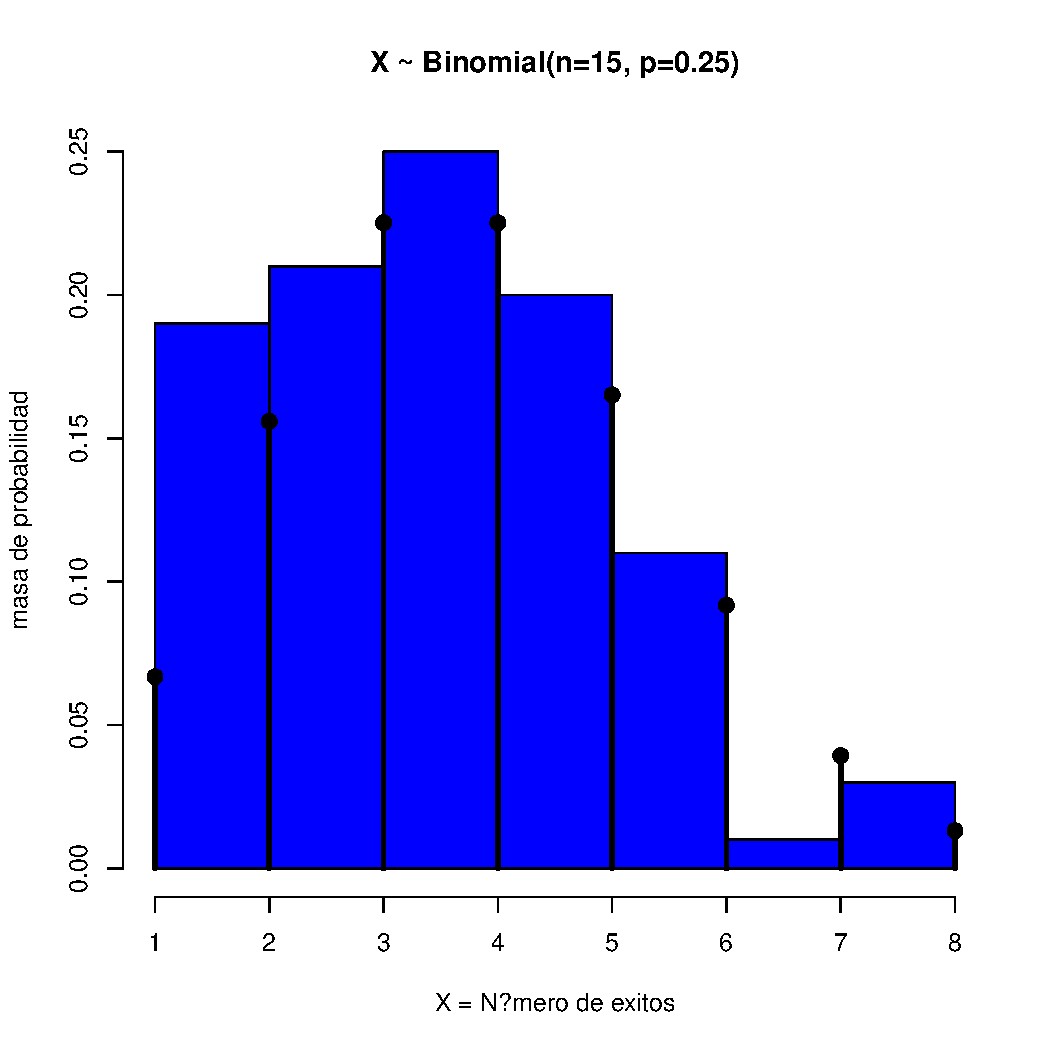
\includegraphics[width=\maxwidth]{figure/unnamed-chunk-29-1} 

\end{knitrout}

\item \textbf{Ejemplo 2:}\\
Generar 100 n\'umeros aleatorios de una distribuci\'on Poisson con 200000 ensayos o pruebas y una probabilidad de \'exito de 3/100000
\begin{knitrout}
\definecolor{shadecolor}{rgb}{0.969, 0.969, 0.969}\color{fgcolor}\begin{kframe}
\begin{alltt}
\hlcom{# Definir los par?metros apropiados}

\hlstd{n} \hlkwb{<-} \hlnum{200000}\hlstd{; p} \hlkwb{<-} \hlnum{3}\hlopt{/}\hlnum{100000}\hlstd{; lambda}\hlkwb{=}\hlstd{n}\hlopt{*}\hlstd{p}

\hlcom{# generar 100 n\textbackslash{}'umeros aleatorios de la distribuci\textbackslash{}'on}

\hlstd{x} \hlkwb{=} \hlkwd{rpois}\hlstd{(}\hlnum{100}\hlstd{, lambda); x}
\end{alltt}
\begin{verbatim}
##   [1]  7  8  4  5  9  4  6 10  7  7  3  8  5  5  3  4  4  3  6  5  2  2  4
##  [24]  3  5  3  5  5  6  8  5  6  5  6  2  8  9 11  6  7  6  9  8  5  3  3
##  [47]  4  9  4  8  7 10  8  7  6  8  6  5  6  7  8  7  6  3 13  6  6  6  7
##  [70]  5  6  4  6  6  5  5  8  5  7 10  7  8  7  4  7  4  3  7  6  6 11  8
##  [93]  5  3  3  6  8  8  5  7
\end{verbatim}
\begin{alltt}
\hlcom{# Histograma para la muestra aleatoria de tama\textbackslash{}~no 100}

\hlkwd{hist}\hlstd{(x,} \hlkwc{main}\hlstd{=}\hlkwd{expression}\hlstd{(}\hlkwd{paste}\hlstd{(}\hlstr{"X ~ Poisson( "}\hlstd{, lambda,} \hlstr{" = 6 )"}\hlstd{)),}
\hlkwc{xlab}\hlstd{=}\hlstr{"X = Numero de eventos a una tasa constante"}\hlstd{,} \hlkwc{ylab}\hlstd{=}\hlstr{"masa de 
probabilidad"}\hlstd{,} \hlkwc{probability}\hlstd{=}\hlnum{TRUE}\hlstd{,} \hlkwc{col}\hlstd{=}\hlstr{"blue"}\hlstd{)}

\hlcom{# Graficar la funci\textbackslash{}'on de probabilidad teorica, use la funci\textbackslash{}'on points()}

\hlstd{xvals}\hlkwb{=}\hlnum{0}\hlopt{:}\hlstd{n;} \hlkwd{points}\hlstd{(xvals,} \hlkwd{dpois}\hlstd{(xvals, lambda),} \hlkwc{type}\hlstd{=}\hlstr{"h"}\hlstd{,} \hlkwc{lwd}\hlstd{=}\hlnum{3}\hlstd{)}
\hlkwd{points}\hlstd{(xvals,} \hlkwd{dpois}\hlstd{(xvals, lambda),} \hlkwc{type}\hlstd{=}\hlstr{"p"}\hlstd{,} \hlkwc{lwd}\hlstd{=}\hlnum{3}\hlstd{)}
\end{alltt}
\end{kframe}
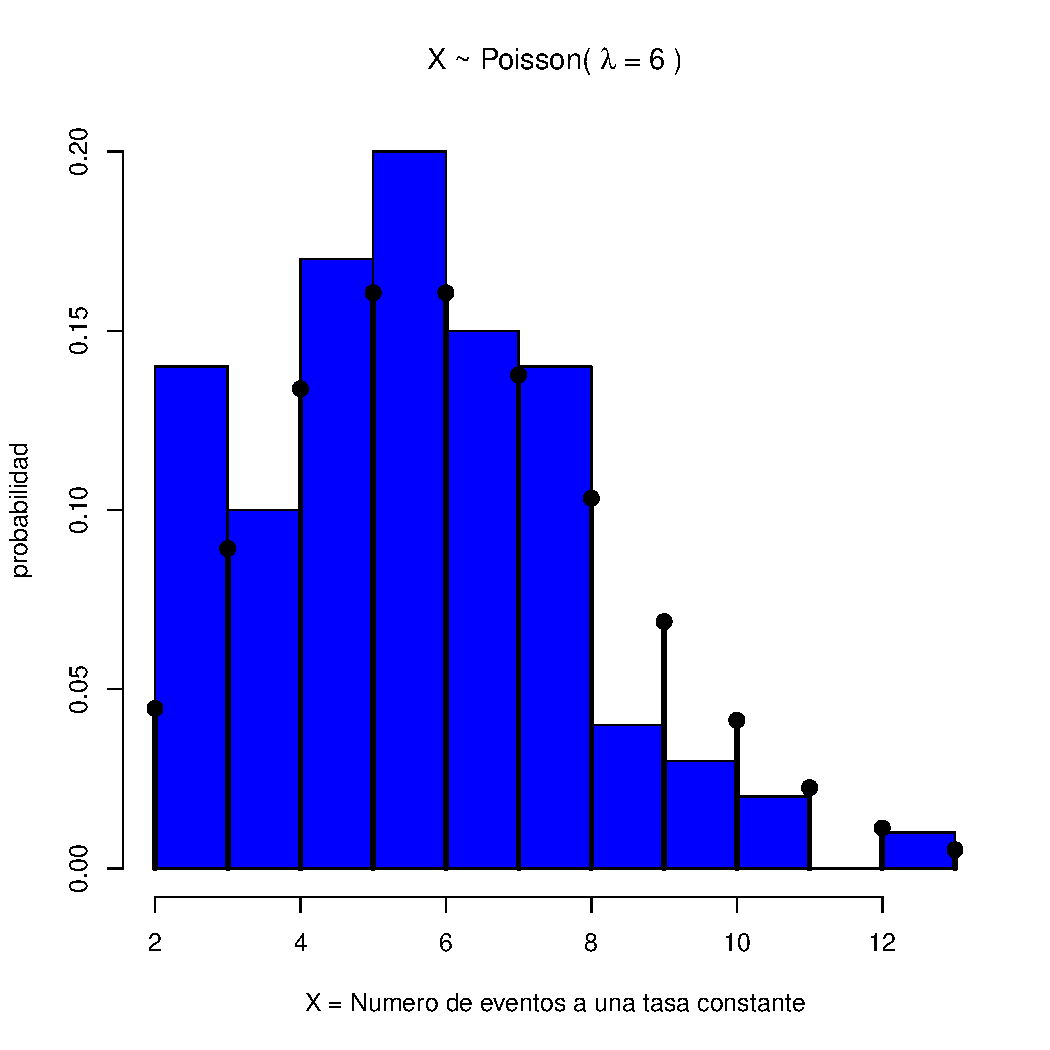
\includegraphics[width=\maxwidth]{figure/unnamed-chunk-30-1} 

\end{knitrout}
\end{itemize}
\end{document}
